\documentclass[conference]{IEEEtran}
\usepackage[utf8]{inputenc}
\usepackage{blindtext, graphicx}
\usepackage{tikz}
\usepackage{tikz}
% we want ER + above/below + left/right
\usetikzlibrary{er,positioning}
\hyphenation{op-tical net-works semi-conduc-tor}

\begin{document}

\title{The usability and buildability of an open source Monitoring Box}

\author{
	\IEEEauthorblockN{Mick Nieman}
	\IEEEauthorblockA{Business IT \& Management\\Amsterdam University\\of Applied Sciences\\
		Wibautstraat 2-4 1091GM Amsterdam\\
		The Netherlands\\
		Mick.Nieman@hva.nl
		}		
	\and
		\IEEEauthorblockN{Pjotr Scholtze}
		\IEEEauthorblockA{Software Engineering \\Amsterdam University\\of Applied Sciences\\
			Wibautstraat 2-4 1091GM Amsterdam\\
			The Netherlands\\
			Pjotr.Scholtze@hva.nl
			}			
		\and
			\IEEEauthorblockN{Heeyeon Joung}
			\IEEEauthorblockA{Electrical Engineering\\Seoul National University\\
			of Science and Technology \\
			Seoul Nowon-gu, Gongneung-dong,\\
			Gongneung-ro 232, South-Korea\\
			Julia.Joung@hva.nl
			}	
		}
	

\maketitle	



\begin{abstract}
This paper is written in commission of the Citizen Data lab from Amsterdam. The main goal of this report is to avoid pitfalls and find solutions for making an open source data-gathering platform. Commissioner of this research is Wouter Meys, Lab Coordinator of the Citizen Data Lab. The reason for this research, along with a developed prototype is the lack of useful environmental data-loggers which also keep track of the GPS-coordinates. This is critical for the Citizen Data Lab when they are, what they call, 'mapping the city'. \\

\end{abstract}

\begin{IEEEkeywords}
Open-source, usability, buildability, environment, data logging
\end{IEEEkeywords}

\IEEEpeerreviewmaketitle

\section{Introduction}
 Researchers nowadays use data to answer the questions asked within their research, that is how research is done. Because of this collecting data for their research is also part of the researchers their task-list and that is not as easy as it seems. Data is collected by researchers doing so called 'data-sprints', this is where a group of people try to collect as much data as possible to do new findings on a certain topic. This is not different for the Citizen Data Lab and their researchers who do research, and back their research, by collecting data through data-sprints. Lately they find their selves struggling collecting the data and most important a specific aspect of their data, the location. For this very reason the development of the Monitoring Box began. The monitoring box tries to hand a solution to the researchers that not only is very convenient but also something researchers can build individually and without any interference of third parties. This way the costs stay low and the usability high. \par
This paper is a result of findings made during the development phase and the testing phase of the prototype of the monitoring box. The paper is written based on the findings and used to be learnt from when further developing the monitoring box. It may also be used by others developing similar open source data gathering platforms.

\subsection{Statement of Purpose}
This has no content yet and needs to be filled in. 

\subsection{Statement of Significance}
This has no content yet and needs to be filled in. 

\section{Research Questions}

\subsection{Overall research question}
What factors contribute to creating an open source, multi-research, sensor geolocation aware, data gathering platform that can be used by the students and researchers from the Makerslab on the Amsterdam University of applied sciences?

\subsection{Sub-questions}
\begin{enumerate}
\item How technical are the students and researchers from the Makerslab on the Amsterdam University of applied sciences?
\begin{enumerate}
\item What documentation is needed and how detailed should it be
\end{enumerate}
\item What improves the usability of the product when taking the structure plane of user experience into account?
\item How can the data be made available such that the students \& researchers from the Minor Makerslab can use it?
\end{enumerate}

\section{Review of literature}
This has no content yet and needs to be filled in. 

\section{Methods}
	To conduct the research a prototype that can be build multiple times is required. Therefore a prototype was created before user studies were preformed. And further modified during the research process. In order to complete the research we carried out the following steps:
	\begin{enumerate}
		\item Identify the use cases of the system.
		\item Generalize the use cases to a generic platform design.
		\item Create prototype.
		\item Research usability concerns.
	\end{enumerate}
	\subsection{Prototype}
		The prototype consists of a base station (a Raspberry Pi) and different sensors (using Arduino's). To make sure that the whole setup stayed modular a translation part (the Arduino's) were used. This design ensures that the base station only needs to know one protocol and does not need to know the individual sensors. ("Designing Multi-Agent Systems around a Programmable Communication Abstraction") Which allows the base station  to focus on using recording the data, managing data storage and making the sensors dynamically attachable.
		\begin{figure}[ht]
			\centering
			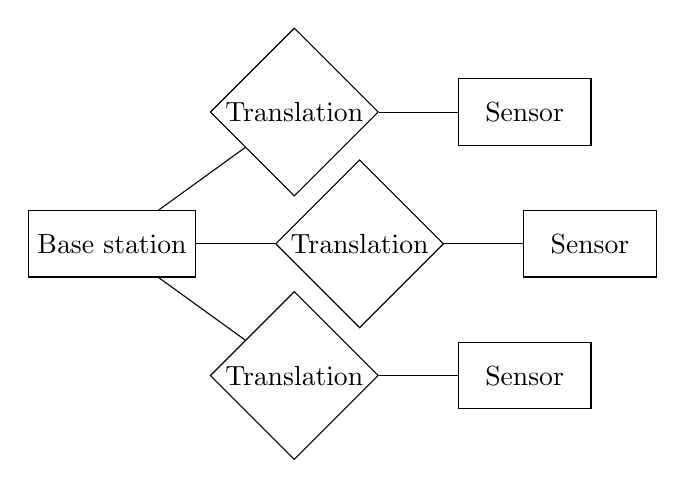
\begin{tikzpicture}[auto,node distance=1cm]
				\node[entity] (node1) {Base station}
								[grow=up,sibling distance=3cm];
				% Now place a relation (ID=rel1)
				\node[relationship] (rel1) [below right = of node1] {Translation};
				\node[relationship] (rel2) [right = of node1] {Translation};
				\node[relationship] (rel3) [above right = of node1] {Translation};
				% Now the 2nd entity (ID=rel2)
				\node[entity] (node2) [right = of rel1]	{Sensor};
				\node[entity] (node3) [right = of rel2]	{Sensor};
				\node[entity] (node4) [right = of rel3]	{Sensor};
				% Draw an edge between rel1 and node1; rel1 and node2
				\path (rel1) edge node {} (node1)
							edge	 node {}	(node2);
				\path (rel2) edge node {} (node1)
							edge	 node {}	(node3);
				\path (rel3) edge node {} (node1)
							edge	 node {}	(node4);
			\end{tikzpicture}
			\caption{Example connection diagram prototype}
		\end{figure}
		\paragraph{Prototype parts}
			\begin{enumerate}
				\item Base station
					\begin{enumerate}
						\item Wifi accesspoint
						\item Web interface
						\item Recording
					\end{enumerate}
				\item Sensors
					\begin{enumerate}
						\item GPS
						\item Temperature and humidity sensor
						\item CO2 sensor (two types)
						\item Heartrate sensor
						\item Galvanic skin response sensor
						\item Camera (PIcam)
					\end{enumerate}
			\end{enumerate}
		\paragraph{Prototype features}
			The base station allows all sensors to be plug and play while on except the Picam. Each sensor can be seen on the web interface or via the screen on the base station. The recordings can only be started via the touchscreen on the base station. Recordings can be downloaded from the web interface or via USB stick that can be mounted on the base station. Every sensor is attached to the base station via USB for ease of use and availability of the devices. An USB hub can easily be used to extend the amount of sensors the base station can handle simultaneously. 
	\subsection{Research}
		In this section is described how each sub question of our main research question is researched. So as to decide the effective method of research we have considered what we needed to do with the research. We considered what should be focused more between breadth and depth or between quantification and qualification and what would be more efficient in empirical research and desk research in each sub question. Along with these considerations, we have came to the following decision. 

		First, to research 'how technical are the students and researchers from the Makerslab on the Amsterdam University of applied sciences?', We let students and researchers from the Makerslab use the Monitoring box. Because we wanted to gain various types of students and researchers in technical point, panels of survey should be breadth. With this we can determine what explanation is needed according to the technical level. So, questions of survey include users' comments so to gain insight in to this. 

		Second, in order to research 'What improves the usability of the product when taking the structure plane of user experience into account?', surveys and desk research are used. And compare this with the shortcomings in usability aspects through existing, similar-functioning platforms and devices. In order to research the Monitoring box in the direction of improving the insufficient aspects of usability.

		Third, in order to research the question 'How can the data be made available such that the students \& researchers from the Minor Makerslab can use it?' desk research is used. We look at other similar cases and consider choosing the most appropriate way of data sharing and how researchers use open source and data gathering platforms.
	\paragraph{Interview setup} The interviews were executed in the following order:
		\begin{enumerate}
			\item Give general introduction to the project to participant.
			\item Let participant assemble hardware and upload software.
			\item During assembly of product observe participant.
			\item Let the participant test their work.
			\item Let participant use the prototype.
			\item Ask participant questions from the survey and ask for general feedback.
		\end{enumerate}
		The interviews were recorded with a camera and notes were made during this interview. Of our team all team members were present, one member controlled the camera, one made notes and one did the presentation.
	\paragraph{Interview participants}
		In order to get an accurate picture of user group, a sample with different backgrounds were chosen. This included students and researchers with different levels of technical skills. The participants of the interviews can be categorized in to the following categories:
		\begin{figure}[ht]
			\centering
			\begin{tabular}{ | l | r | l | }
				\hline
				Type			& Amount	& Description \\ \hline \hline
				Researcher		& 2			& Different technical levels* \\ \hline
				Master-students	& 0			& Did not take part \\ \hline \hline
				Student			& 4			& See figure ... for details \\ \hline \hline
				Total			& 6			& \\ \hline
			\end{tabular}
			\caption{General distribution of participants}
		\end{figure}\\
		The master students were unfortunately unavailable for our research. The student group can be sub divided into different sub-categories:
		\begin{figure}[ht]
			\centering
			\begin{tabular}{ | l | r | l | }
				\hline
				Type					& Amount \\ \hline \hline
				Business IT				& 1 \\ \hline
				Game design				& 1 \\ \hline
				Software engineering	& 2 \\ \hline
				Design					& 1? \\ \hline \hline
				Total					& 4 \\ \hline
			\end{tabular}
			\caption{Major of the participating students}
		\end{figure} \\
		This shows a users from varying backgrounds participated in the research. However unfortunately because of time and resources we had limitation in size of this group
\section{Results}
\begin{enumerate}
\item How technical are the students and researchers from the Makerslab on the Amsterdam University of applied sciences?
\begin{enumerate}
\item What documentation is needed and how detailed should it be
\end{enumerate}

 We created 'Manual Monitoring Box' documentation based on the process of building the Monitoring Box. We started with a list of parts we used and a brief introduction to them. Since their background knowledge is different, we explain first how to install the software, how to upload it to Arduino, and how to get the results. And for each sensor, we describe how the Arduino and the sensor should be connected by schematic and letter. We invited two researchers and three students from the Amsterdam University of applied sciences and require them building the Monitoring box based on our 'Manual Monitoring Box'. \\
\begin{enumerate}
\item Researcher A

The researcher encountered the following problems during the interview.\\

		First, she does not know how to use breadboard. To create a Galvanic Skin Response sensor, user have to connect the Arduino Nano, resistor, and several wires. However, these connections are not just one-to-one connections, they require multiple connections. So in order to succeed, user must understand the structure of the breadboard. The manual did not explain the structure of the breadboard, and the researcher had difficulty with it.\\
		Second, she wanted more specify information about cable connections.\\
		 		
The researcher has mentioned that we need the following elements in the document.\\

		First, she suggested that we mention in the manual how to use breadboard and the structure of breadboard. \\
		Second, she suggested that we add more information about Arduino nano and Arduino uno.\\
		Third, she said the manual does not focus in Dutch, but English. \\
		
\item Researcher B

Researcher B knows quite a bit of software and has little knowledge of hardware. The researcher encountered the following problems during the interview.\\

		First, he feels there are something unclear about the schematic. He pointed out that the schematic pin number is missing. The pin number is too small to specify, so he was uncomfortable with rebuilding.\\
		Second, he was wondering about the difference between the two CO2 sensors. The manual only briefly specifies the name and characteristics of each sensor, but the difference between the two sensors is not specified in detail.\\
		Third, he did not know how to use the breadboard.\\

The researcher has mentioned that we need the following elements in the document.\\

		First, he suggested that we mention in the manual when to upload and where to see the results. \\
		Second, he suggested links to tutorials about breadboard.\\
		Third, he suggested that we put the technical names in the shopping list\\
		Forth, he suggested that we explain in the manual which part is wrong for each error message.\\

\item Student A

Student A is majoring in Computer Science and has  quite some experience in Arduino. The student A encountered the following problems during the interview.\\

		First, he confused about the GPS and Arduino nano. He was confused because the GPS and Arduino nano have similar size and similar color.\\
		Second, he had difficulty reading the schematics. The letters in the schematics are too small to read, and it took some time to find out what was written on the next page.\\

The researcher has mentioned that we need the following elements in the document.\\

		First, he suggested to write the steps in bold.\\
		Second, he suggested adjusting the order of text and schematics. He mentioned that it took a some time to find that there is a text which explain schematics. 

\item Student B

Student B is majoring in Game development and has  quite some experience in Arduino. He replied that his technical level is a hobby in the hardware and professional in the software. The student B pointed out the following during the interview.\\

		First, the manual is really easy but it did not state which arduino sketch is necessary to complete.
		Second, pictures should represent the real life device. Heart rate sensor in the schematic and real heart rate sensor look different.

\item Student C

Student C is majoring in Computer science and has  quite some experience in Arduino. The student C pointed out the following during the interview.\\

		First, the Galvanic Skin Response schematic is not clear. The Galvanic Skin Response chapter is not indepth with the explanation of how to connect everything.\\
		Second, he ask how can he test the sensors.\\
		Third, he suggested that we explain more information about cable.\\

\end{enumerate}

 
\item What improves the usability of the product when taking the structure plane of user experience into account?

In interaction design in the structure plane of user experience, users must communicate correctly to the monitoring box and the monitoring box must deliver the information that the user wants immediately and accurately. In this respect, the Monitoring box has a touch screen and we have added four menus in this screen so that when the user has the information they want, they can instantly check the menu. The home screen shows what percentage of the storage capacity is in use and if users select 'Sensor' menu from the Monitoring Box, users can see the currently connected sensor. And if users select 'Wifi' menu from Monitoring Box, users can confirm the Wifi name and password.//
In information architecture in the structure plane of user experience, it should facilitate intuitive access to data. So we used wireless WiFi so that we could check the information if we had an internet capable device. And with a single push of a button on the Internet Web site, users are able to download the data of the sensors they had recorded at a glance. In addition, the monitoring box screen design allows intuitive use of the menu.
\\

\item How can the data be made available such that the students \& researchers from the Minor Makerslab can use it?
\begin{enumerate}
\item In the Monitoring Box
\begin{enumerate}
\item Screen
\begin{enumerate}
\item Main menu

 In the main menu, there are one bar and four menus. The bar tells users how much storage they have used. This percentage allows the user to see how much memory is left on the SD card and to control usage. Each menu button has a label for explaining its purpose.\\
\item Record

 Users can start recording by pushing this menu. In addition, they can see which sensors are recording while recording.\\
\item Sensor

 In the Sensor menu, user can see a list of currently connected sensors. It is good to check before users know that the users are sure of the connection.\\
\item WiFi

 WiFi name and password can be found in this menu. Users do not need to remember or write down Monitoring Bx WiFi name and password.\\
\end{enumerate}

\end{enumerate}

\item In the Website
\begin{enumerate}
\item Wireless connect to Web page

 The data that users have recorded can be downloaded at once. We use the wireless data transmitter to view the data, even if users do not have a certain cable, users can see data only if they have a Wi-Fi enabled devices such as laptop computer or smart phone. \\
 A few simple steps are required for users to connect their Monitoring Box to the Web page. First, turn on a Wi-Fi enabled devices and connect Monitoring box Wi-Fi. The Monitoring box is equipped with Wi-fi function and the WiFi name and password can be found in the menu on the monitoring box screen. Second, if you complete the first step, users can go to the monitoring box website by typing 'monitoring.box:5000' in the web site address.\\

\item Download the recorded information

 After users access a website, they can see and download the data which they have recorded. The downloadable format is CSV(Comma Separated Value). Because it is truncated in the form of a comma, it can be read not only as a text file but also as an Excel file. When users open CSV file in Excel, the user can view and store the sorted data in sequence.\\

\item Graph

 Users can view a list of currently connected sensors in real time on the web page and a graph of their sensor values. Users can easily access data and see the data at a glance.\\

\end{enumerate}
\end{enumerate}
 
\end{enumerate}

\section{Discussion}
This has no content yet and needs to be filled in. 

\section{Limitations}
This has no content yet and needs to be filled in. 

\section{Conclusion}
This has no content yet and needs to be filled in. 

\bibliography{Research_Report_Monitoring_Box}

\appendices
\section{Baseline of questions asked during user tests}
\begin{enumerate}
\item Which field do you have expertise in?
\item What is your level of technology in hardware?
\item What is your level of technology in software
\item How does the explanation of the parts in the manual help you using the monitoring box?
\item Do you think developers with similar technical levels can make and use the monitoring box as well?\item What could be improved when looking at the monitoring box?
\item What could be improved when looking at the manual?
\end{enumerate}

\end{document}
